\section{Finite Markov Decision Processes}

\subsection{The Agent-Environment Interface}
\begin{figure}[h!]
	\centering
	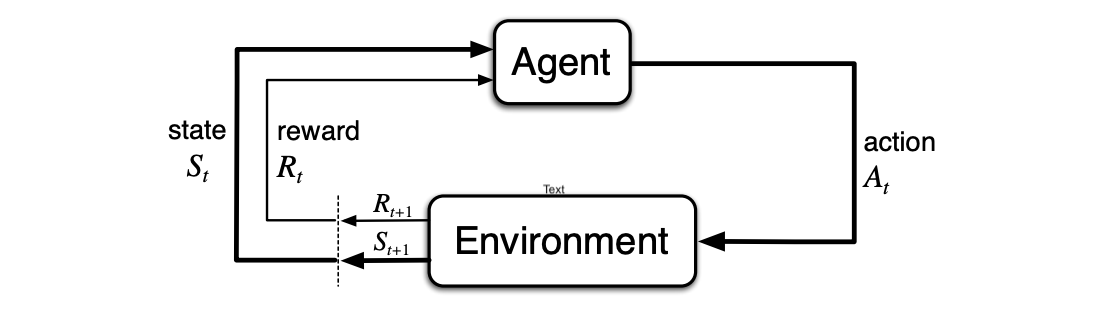
\includegraphics[width=\textwidth]{/chapter3_1}
	\caption{The agent-environment interface in reinforcement learning}
	\label{fig:agent-environment}
\end{figure}

\begin{itemize}
	\item At each timestep the agent implements a mapping from states to probabilities of selecting a possible action. The mapping is called the agents \textit{policy}, denoted \(\pi\), where \(\pi(a | s)\) is the probability of the agent selecting actions a in states.
	\item In general, actions can be any decision we want to learn how to make, and states can be any interpretation of the world that might inform those actions.
	\item The boundary between agent and environment is much closer to the agent than is first intuitive. E.g. if we are controlling a robot, the voltages or stresses in its structure are part of the environment, not the agent. Indeed reward signals are part of the environment, despite very possibly being produced by the agent e.g. dopamine.
\end{itemize}

\subsection{Goals and Rewards}
The \textit{reward hypothesis}:
\begin{displayquote}
	All we mean by goals and purposes can be well thought of as the maximization of the expected value of the cumulative sum of a received scalar signal (called reward).
\end{displayquote}

The reward signal is our way of communicating to the agent what we want to achieve not how we want to achieve it.

\subsection{Returns and Episodes}
The return \(G_t\) is the sum of future rewards:

\begin{equation}
	G_t = R_{t+1} + R_{t+2} + R_{t+3} + \cdots + R_t
\end{equation}

\begin{itemize}
	\item This approach makes sense in applications that finish, or are periodic. That is, the agent-environment interaction breaks into \textit{episodes}.
	\item We call these systems \textit{episodic tasks}. e.g playing a board game, trips through a maze etc.
	\item Notation for state space in an episodic task varies from the conventional case (\(s \in \mathcal{S}\)) to (\(s \in \mathcal{S^+}\))
	\item The opposite, continuous applications are called \textit{continuing tasks}.
	\item For these tasks we use \textit{discounted returns} to avoid a sum of returns going to infinity.
\end{itemize}

\begin{equation}
	G_t = R_{t+1} + \gamma R_{t+2} + \gamma^2 R_{t+3} + \cdots = \sum_{k=0}^{\infty} \gamma^k R_{t+k+1} 
\end{equation}

If the reward is a constant + 1 at each timestep, cumulative discounted reward $G_t$ becomes:

$
G_t = \sum_{k=0}^{\infty} \gamma^k = \frac{1}{1 - \gamma}
$

\textit{Discounting} is a crucial topic in RL. It allows us to store a finite value of any state (summarised by its expected cumulative reward) for continuous tasks, where the non-discounted value would run to infinity. 

\subsection{Unified Notation for Episodic and Continuing Tasks}
\begin{equation}
	G_t = \sum_{k=0}^{T-t-1} \gamma^k R_{t+k+1} 
\end{equation}

\subsection{The Markov Property}
A state signal that succeeds in retaining all relevant information about the past is \textit{Markov}. Examples include:
\begin{itemize}
\item A cannonball with known position, velocity and acceleration
\item All positions of chess pieces on a chess board.
\end{itemize}

In normal causal processes, we would think that our expectation of the state and reward at the next timestep is a function of all previous states, rewards and actions, as follows:

\begin{equation}
	Pr \{R_{t+1} = r, S_{t+1} = s' | S_0, A_0, R_1, \ldots, S_{t-1}, A_{t-1}, R_t, S_t, A_t\}  
\end{equation}

If the state is Markov, however, then the state and reward right now completely characterizes the history, and the above can be reduced to:

\begin{equation}
p(s', r | s, a) = Pr \{R_{r+1} = r, S_{t+1} = s' | S_t, A_t\}
\end{equation}

\begin{itemize}
\item Even for non-Markov states, it is appropriate to think of all states as at least an approximation of a Markov state.
\item Markov property is important in RL because decisions and values are assumed to be a function only of the current state.
\item Most real scenarios are unlikely to be Markov. In the example of controlling HVAC, the HVAC motor might heat up which affects cooling power and we may not be tracking that temperature. It is hard for a process to be Markov without sensing all possible variables.
\end{itemize}

\subsection{Markov Decision Process (MDP)}
Given any state and action s and a, the probability of each possible pair of next state and reward, s', r is denoted:

\begin{equation}
p(s', r | s, a) = Pr \{R_{r+1} = r, S_{t+1} = s' | S_t, A_t\}
\end{equation}

We can think of \(p(s', r | s, a)\) as the dynamics of our MDP, often called the \textit{transition function}–it defines how we move from state to state given actions. 

\subsection{Policies and Value Functions}
\begin{itemize}
\item Value functions are functions of states or functions of state-value pairs.
\item They estimate how good it is to be in a given state, or how good it is to perform a given action in a given state.
\item Given future rewards are dependent on future actions, value functions are defined with respect to particular policies as the value of a state depends on the action an agent takes in said state.
\item A \textit{policy} is a mapping from states to probabilities of selecting each possible action.
\item RL methods specify how the agent's policy changes as a result of its experience.
\item For MDPs, we can define nu-pi(s) formally as:
\end{itemize}

\begin{equation}
v_\pi(s) = \mathbb{E}_\pi \left[G_t | S_t = s \right] = \mathbb{E}_\pi \left[\sum_{k=0}^{\infty} \gamma^k R_{t+k+1} | S_t = s\right]
\end{equation}

i.e. the expected future rewards, given state \(S_t\), and policy \(\pi\). We call \(v_\pi(s)\)the \textbf{state value function for policy \(pi\)}. Similarly, we can define the value of taking action \(a\) in state \(s\) under policy \(\pi\) as:

\begin{equation}
q_\pi(s,a) = \mathbb{E}_\pi \left[G_t | S_t = s, A_t = a \right] = \mathbb{E}_\pi \left[\sum_{k=0}^{\infty} \gamma^k R_{t+k+1} | S_t = s, A_t = a \right]
\end{equation}

i.e. the expected value, taking action \(a\) in state \(s\) then following policy \(\pi\).
\begin{itemize}
\item We call \(q_\pi\) the \textbf{action-value function for policy \(\pi\)}
\item Both value functions are estimated from experience.
\end{itemize}

A fundamental property of value functions used throughout reinforcement learning and dynamic programming is that they satisfy recursive relationships similar to that which we have already established for the return. This recursive relationship is characterised by the \textbf{Bellman Equation}:

\begin{equation}
v_\pi(s) = \sum_{a} \pi(a|s) \sum_{s',r} p(s', r | s, a) \left[r + \gamma v_\pi(s')\right]
\end{equation}

This recursion looks from one state through to all possible next states given our policy and the dynamics as suggested by \ref{fig:backup}:
\begin{figure}[h!]
	\centering
	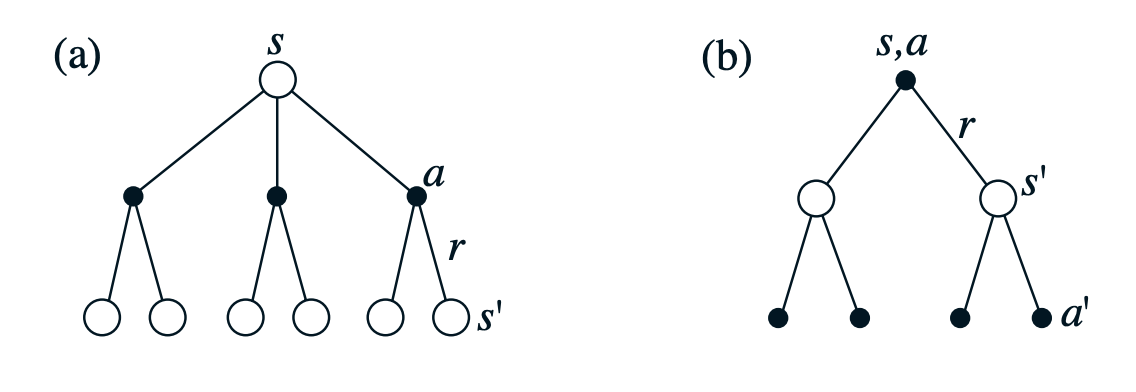
\includegraphics[width=0.25\textwidth]{/chapter3_2}
	\caption{Backup diagrams for \(v_\pi\) and \(q_\pi\)}
	\label{fig:backup}
\end{figure}

\subsection{Optimal Policies and Value Functions}
\begin{itemize}
\item A policy \(\pi '\) is defined as better than policy pi if its expected return is higher for all states.
\item There is always AT LEAST one policy that is better than or equal to all other policies - this is the \textit{optimal policy}.
\item Optimal policies are denoted \(\pi*\)
\item Optimal state-value functions are denoted \(v*\)
\item Optimal action-value functions are denoted \(q*\)
\item We can write \(q*\) in terms of \(v*\):
\end{itemize}

\begin{equation}
q_*(s,a) = \mathbb{E} \left[R_{t+1} + \gamma v_*(S_{t+1}) | S_t = s, A_t = a \right]
\end{equation}

We can adapt the Bellman equation to achieve the Bellman optimality equation, which takes two forms. Firstly for \(v_*\):
\begin{equation}
v_*(s) = \max_{a \in \mathcal{A}(s)} \sum_{s',r} p(s', r | s, a) \left[r + \gamma v_*(s')\right]
\end{equation}
and secondly for \(q_*\):
\begin{equation}
q_*(s) = \sum_{s',r} p(s', r | s, a) \left[r + \gamma \max_{a'} q_*(s', a') \right]
\end{equation}

\begin{itemize}
\item Using \(v*\) the optimal expected long term return is turned into a quantity that is immediately available for each state. Hence a one-step-ahead search, acting greedily, yield the optimal long-term actions.
\item Fully solving the Bellman optimality equations can be hugely expensive, especially if the number of states is huge, as is the case with most interesting problems.
\item Solving the Bellman optimality equation is akin to exhaustive search. We play out \textit{every} possible scenario until the terminal state and collect their expected reward. Our policy then defines the action that maximises this expected reward. 
\item In the continuous case the Bellman optimality equation is unsolvable as the recursion on the next state's value function would never end.
\end{itemize}

\subsection{Optimality and Approximation}
\begin{itemize}
	\item We must approximate because calculation of optimality is too computationally intense.
	\item A nice way of doing this, is allowing the agent to make sub-optimal decisions in scenarios it has low probability of encountering. This is a trade off for being optimal in situations that occur frequently.
\end{itemize}

\subsection{Key Takeaways}


\subsection{Exercises}
\subsubsection{Exercise 3.1}
\textbf{Q}\\
Devise three example tasks of your own that fit into the MDP framework, identifying for each its states, actions, and rewards. Make the three examples as different from each other as possible. The framework is abstract and flexible and can be applied in many different ways. Stretch its limits in some way in at least one of your examples.\\

\textbf{A}\\
\begin{enumerate}
	\item \textit{Golf: Putting}\\
	\begin{itemize}
		\item State: Coordinates of ball; coordinates of hole; x,y,z contour plot of green; grass length; grass type; wind speed; wind direction; ball type; putter type.
		\item Actions: (X, Y) direction of aim; length of stroke
		\item Rewards: -1 for each unit of distance from hole
	\end{itemize}
	\item \textit{Optimizing investment portfolio}
	\begin{itemize}
		\item State: Investment in each company; cash balance; \% return over last minute/hour/day/week/month/year
		\item Actions: For each investment: buy (discretized by some cash interval), sell (discretized by some cash interval), stick
		\item Rewards: +1 for each £ return per day 
	\end{itemize}
	\item \textit{Shoe-tying robot}
	\begin{itemize}
		\item State: Coordinates of laces; coordinates of robot arms/joints
		\item Actions: Grip pressure on laces; adjust position of arms to coordinates x,y,z
		\item Rewards: -1 for unit of shoe displacement from foot once tied.
	\end{itemize}
\end{enumerate}

\subsubsection{Exercise 3.2}
\textbf{Q}\\
Is the MDP framework adequate to usefully represent all goal-directed learning tasks? Can you think of any clear exceptions? \\

\textbf{A}\\
The MDP framework fails when the state cannot be fully observed. For example, one may try to control the temperature of a house using a state space represented by one thermometer in one room. Our agent would control the temperature observed by that thermometer well, but would be blind to temperatures that aren't measured by said thermometer elsewhere in the house.

\subsubsection{Exercise 3.3}
\textbf{Q}\\
Consider the problem of driving. You could define the actions in terms of the accelerator, steering wheel, and brake, that is, where your body meets the machine. Or you could define them farther out—say, where the rubber meets the road, considering your actions to be tire torques. Or you could define them farther in—say, where your brain meets your body, the actions being muscle twitches to control your limbs. Or you could go to a really high level and say that your actions are your choices of where to drive. What is the right level, the right place to draw the line between agent and environment? On what basis is one location of the line to be preferred over another? Is there any fundamental reason for preferring one location over another, or is it a free choice?\\

\textbf{A}\\
There's a trade-off between state-action space complexity, computational expense and accuracy. If we draw the boundary at the brain we would create a state-action space contingent on the number of neurons in the brain and their interplay with physical actions like turning the steering wheel; too large to be stored or computed efficiently. Equally, if we draw the boundary at the \textit{journey} level, then we miss the detail required to act on second-by-second state changes on the road that could lead to a crash. The fundamental limiting factor in this selection is whether the goal can be achieved safely at your chosen layer of abstraction, indeed this feels like one of the tasks of engineering more widely.

\subsubsection{Exercise 3.4}
\textbf{Q}\\
Give a table analogous to that in Example 3.3, but for \(p(s0, r|s, a)\). It should have columns for \(s, a, s', r,\) and \(p(s0, r|s, a)\), and a row for every 4-tuple for which \(p(s0, r|s, a) > 0\).\\

\textbf{A}\\
\begin{table}[]
	\begin{tabular}{llll|l}
		\(s\) & \(a\) & \(s'\) & \(r\) & p(\(s, r, | s, a\)) \\ \hline
$\mathnormal{high}$		& $ \mathnormal{search}$     & $\mathnormal{high} $       & \(r_{\mathnormal{search}}\)       &   \(\alpha\)   \\
$\mathnormal{high}$		&  $\mathnormal{search}$     &  $\mathnormal{low}$      &   \(r_{\mathnormal{search}}\)     &  \((1-\alpha)\)                   \\
$\mathnormal{low}$		&  $\mathnormal{search}$     & $\mathnormal{high}$       & -3      & \((1-\beta)\)                    \\
$\mathnormal{low}$		&  $\mathnormal{search}$    & $\mathnormal{low} $       &  \(r_{\mathnormal{search}}\)      & \(\beta\)                     \\
$\mathnormal{high}$		&  $\mathnormal{wait}$     & $\mathnormal{high}$       & \(r_{\mathnormal{wait}}\)       &   1   \\
$\mathnormal{low}$		&  $\mathnormal{wait}$   & $\mathnormal{low}$       &  \(r_{\mathnormal{wait}}\)      &  1  \\
$\mathnormal{low}$		&  $\mathnormal{recharge}$   & $\mathnormal{high}$       &  0      &   1    \\   
	\end{tabular}
\end{table}

As there is no probability distribution over the rewards (i.e. for each state-action pair, the agent receives some reward with \(p(r) = 1\))), \(p(s', r | s, a) = p(s' | s, a)\).\\

\subsubsection{Exercise 3.5}
\textbf{Q}\\
The equations in Section 3.1 are for the continuing case and need to be modified (very slightly) to apply to episodic tasks. Show that you know the modifications needed by giving the modified version of (3.3). \\

\textbf{A}\\
Equation 3.3 from section 3.1 is:

\begin{equation}
	\sum_{s' \in S} \sum_{r \in R} p(s', r | s, a) = 1, \forall s \in S, a \in A(s)
\end{equation}

for episodic tasks this becomes:

\begin{equation}
\sum_{s' \in S^+} \sum_{r \in R} p(s', r | s, a) = 1, \forall s \in S, a \in A(s)
\end{equation}

\subsubsection{Exercise 3.6}
\textbf{Q}\\
Suppose you treated pole-balancing as an episodic task but also used discounting, with all rewards zero except for 1 upon failure. What then would the return be at each time? How does this return differ from that in the discounted, continuing formulation of this task? \\

\textbf{A}\\
In the discounted, episodic version of the pole-balancing task, the return after each episode is:

\begin{equation}
	G_t = -\gamma^{T-t}
\end{equation}

where \(T\) is the timestep at which the episode ends i.e. the task is failed. In the continuining case the cumulative return is:

\begin{equation}
G_t = -\sum_{K\in\mathcal{K}} \gamma^{K-1}
\end{equation}

where \(\mathcal{K}\) is the set of times where the task is failed. Note this reward will increase in the long run, irrespective of improved performance. Designing this as a continuous task does not therefore make sense here.

\subsubsection{Exercise 3.7}
\textbf{Q}\\
Imagine that you are designing a robot to run a maze. You decide to give it a reward of +1 for escaping from the maze and a reward of zero at all other times. The task seems to break down naturally into episodes—the successive runs through the maze—so you decide to treat it as an episodic task, where the goal is to maximize expected total reward (3.7). After running the learning agent for a while, you find that it is showing no improvement in escaping from the maze. What is going  wrong? Have you effectively communicated to the agent what you want it to achieve?\\

\textbf{A}\\
We have designed the reward such that it receives +1 only once it has exited the maze, and are therefore not incentivising it to learn how to exit the maze faster. To do so, we would need to provide a negative reward proportional to time in the maze e.g. -1 per timestep.

\subsubsection{Exercise 3.8}
\textbf{Q}\\
Suppose \(\gamma\) = 0.5 and the following sequence of rewards is received R1 = -1, R2 = 2, R3 = 6, R4 = 3, and R5 = 2, with T = 5. What are \(G_0, G_1, \ldots, G_5\)? Hint: Work backwards.\\

\textbf{A}\\
We know:
$
G_t = R_{t+1} + \gamma G_{t+1}
$
Therefore, for the terminal state:
$
G_5 = 0
$
then:
$
G_4 = 2 +  (0.5 \times 0) = 2\\
G_3 = 3 + (0.5 \times 2) = 4\\
G_2 = 6 + (0.5 \times 4) = 8\\
G_1 = 2 + (0.5 \times 8) = 6\\
G_0 = -1 + (0.5 \times 6) = 2\\
$
Note our expected cumulative reward \(G_t\) depends greatly on our instant reward \(G_{t+1}\) because it is not  discounted.

\subsubsection{Exercise 3.9}
\textbf{Q}\\
Suppose \(\gamma\)  = 0.9 and the reward sequence is $R_1$ = 2 followed by an infinite sequence of 7s. What are $G_1$ and $G_0?$\\

\textbf{A}\\
We know that if the reward is an infinite series of 1s, $G_t$ is:
$
G_t = \sum_{k=0}^{\infty} \gamma^k = \frac{1}{1-\gamma}
$

So for an infinite series of 7s this becomes:
$
G_t = \sum_{k=0}^{\infty} \gamma^k = \frac{7}{0.1}
$

Therefore:
\begin{align}
G_0 &= 2 + \frac{7}{0.1} \\
&= 72
\end{align}
and 
\begin{align}
G_1 &= 7 + \frac{7}{0.1} \\
&= 77
\end{align}


\subsubsection{Exercise 3.10}
\textbf{Q}\\
Prove the second equality in (3.10). \\

\textbf{A}\\
Skipped.

\subsubsection{Exercise 3.11}
\textbf{Q}\\
If the current state is $S_t$, and actions are selected according to a stochastic policy \(\pi\), then what is the expectation of $R_{t+1}$ in terms of $\pi$ and the four-argument function \(p\) (3.2) \\

\textbf{A}\\
$
\mathbb{E}_\pi[R_{t+1} | s_t] = \sum_{a} \pi(a | s) \sum_{s'} \sum_{r} p(s', r | s, a) [r] 
$

\subsubsection{Exercise 3.12}
\textbf{Q}\\
Give an equation for $v_\pi$ in terms of $q_\pi$ and $\pi$. \\

\textbf{A}\\
The state value function \(v_\pi\) is equal to the expected cumulative return from that state given a distribution of actions. The state-action value function \(q_\pi\) is the value of being in a state and taking a deterministic action. Therefore the state value function is the weighted sum of the state action value function, with the weights equal to the probabilities of selecting each action:
$
v_\pi = \sum_{a} \pi(a | s) q_\pi(s,a) 
$

\subsubsection{Exercise 3.13}
\textbf{Q}\\
Give an equation for $q_\pi$ in terms of $v_\pi$ and the four-argument $p$.  \\

\textbf{A}\\
Given an action $a$, the state-action value function is the probability distributions over the possible next states and rewards from that action, times the one-step reward and the discounted state value function at the next timestep:
$
q_\pi = \sum_{s' \in \mathcal{S}} \sum_{r \in \mathcal{R}} p(s', r | s, a) [r + \gamma v_\pi(s_{t+1})]
$

\subsubsection{Exercise 3.14}
\begin{figure}[h!]
	\centering
	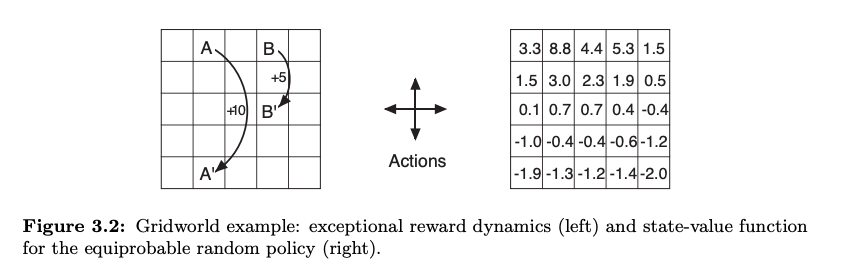
\includegraphics[width=\textwidth]{/ex3.14}
	\caption{Gridworld example for ex. 3.14}
	\label{fig:3.14}
\end{figure}

\textbf{Q}\\
The Bellman equation (3.14) must hold for each state for the value function $v_\pi$ shown in Figure 3.2 (right) of Example 3.5. Show numerically that this equation holds for the center state, valued at +0.7, with respect to its four neighbouring states, valued at +2.3, +0.4, 0.4, and +0.7. (These numbers are accurate only to one decimal place.) .  \\

\textbf{A}\\
Bellman equation for $v_\pi$ is:
\begin{equation}
v_\pi(s) = \sum_{a} \pi(a | s) \sum_{s', r} p(s', r | s, a) [r + \gamma v_\pi(s')] 
\end{equation}
for the centre square in Figure \ref{fig:3.14} we get the following:
\begin{align}
v_\pi(s) &= 0.25 \left[0.9 \times 2.3\right] + 0.25 \left[0.9 \times 0.7\right] + 0.25 \left[0.9 \times 0.4\right] + 0.25 \left[0.9 \times -0.4\right] \\
			&= 0.68 \approx 0.7 
\end{align}

\subsubsection{Exercise 3.15}
\textbf{Q}\\
In the gridworld example, rewards are positive for goals, negative for running into the edge of the world, and zero the rest of the time. Are the signs of these rewards important, or only the intervals between them? Prove, using (3.8), that adding a constant $c$ to all the rewards adds a constant, $v_c$, to the values of all states, and thus does not affect the relative values of any states under any policies. What is $v_c$ in terms of $c$ and $\gamma$? \\

\textbf{A}\\
Part 1): The sign of the reward is of no consequence, it is indeed the interval between each reward that drives behaviour.\\
Part 2): Equation 3.8 is as follows:
\begin{equation}
G_t = \sum_{k=0}^{\infty} \gamma^k R_{t+k+1}
\end{equation}
when we add a constant $c$ to all rewards this becomes:
$
G_t = \sum_{k=0}^{\infty} \gamma^k [R_{t+k+1} + c]
G_t = \frac{R_{t+k+1}}{1 - \gamma} + \frac{c}{1 - \gamma}
$

Expected cumulative reward from every state receives a constant additive term. \(v_c\) in terms of $c$ and $\gamma$ is:
\begin{align}
v_c &= \mathbb{E}\left[\sum_{k=0}^{\infty}\gamma^k c\right]\\
&= \frac{c}{1 - \gamma}
\end{align}

\subsubsection{Exercise 3.16}
\textbf{Q}\\
Now consider adding a constant $c$ to all the rewards in an episodic task, such as maze running. Would this have any effect, or would it leave the task unchanged as in the continuing task above? Why or why not? Give an example. \\

\textbf{A}\\
In the episodic task adding a constant to all rewards does affect the agent. Since the cumulative reward now depends on the length of the episode ($G_t = \sum_{k=t+1}^{T} \gamma^{k-t-1}R_k $), timesteps that incur positive rewards act to lengthen the episode and vice versa. In the maze running example, we may have chosen to give the agent -1 reward at each timestep to ensure it completes the task quickly. If we add $c=2$ to every reward such that the reward at each timestep is now positive, the agent is now incentivised to not find the exit, and continue collecting intermediate rewards indefinitely. 

\subsubsection{Exercise 3.17}
\begin{figure}[h!]
	\centering
	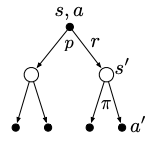
\includegraphics[width=\textwidth]{/ex3.17}
	\caption{Backup diagram for $q_\pi$}
	\label{fig:3.17}
\end{figure}
\textbf{Q}\\
What is the Bellman equation for action values, that is, for $q_\pi$? It must give the action value $q_\pi(s, a)$ in terms of the action values, $q_\pi(s0, a0)$, of possible successors to the state–action pair $(s, a)$. Hint: The backup diagram to the right corresponds to this equation. Show the sequence of equations analogous to (3.14), but for action values.

\textbf{A}\\
\begin{align}
q_\pi(s,a) &= \mathbb{E}_\pi[G_t | S_t = s, A_t = a] \\
&= \mathbb{E}_\pi[R_{t+1} + \gamma G_{t+1} | S_t = s, A_t = a] \\
&= \sum_{s', r} p(s', r | s, a) [r + \gamma \mathbb{E}_\pi[G_{t+1} | s', a']] \\
&= \sum_{s', r} p(s', r | s, a) [r + \gamma q_\pi(s', a')] \\
\end{align}

\subsubsection{Exercise 3.18}
\textbf{Q}\\
\begin{figure}[h!]
	\centering
	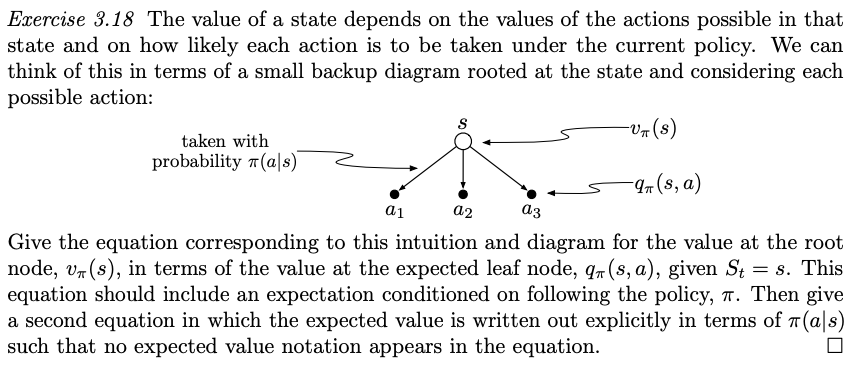
\includegraphics[width=\textwidth]{/ex3.18}
	\label{fig:3.18}
\end{figure}

\textbf{A}\\
\begin{equation}
v_\pi(s) = \mathbb{E}_\pi \left[q_\pi(s,a)\right] \\
v_\pi(s) = \sum_{a} \pi(a|s) q_\pi(s,a)
\end{equation}

\subsubsection{Exercise 3.19}
\textbf{Q}\\
\begin{figure}[h!]
	\centering
	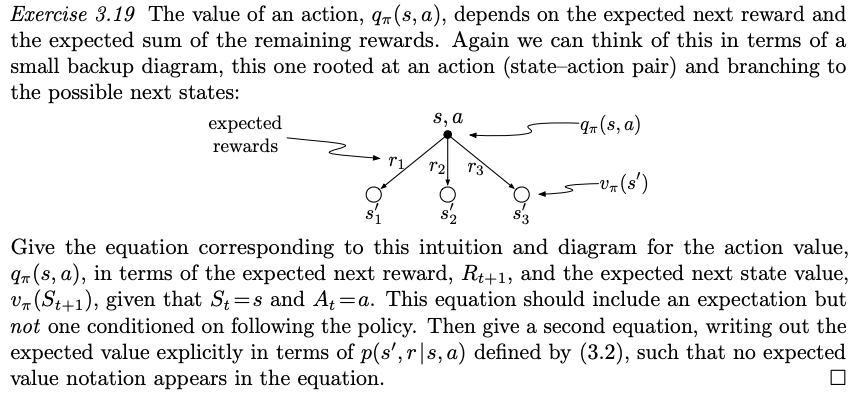
\includegraphics[width=\textwidth]{/ex3.19}
	\label{fig:3.19}
\end{figure}

\textbf{A}\\
\begin{align}
q_\pi(s, a) &= \mathbb{E} \left[R_{t+1} + v_\pi(s') | S_{t} = s)\right] \\
&= \sum_{s', r} p(s', r | s, a) [r +v_\pi(s')]\\
\end{align}

\subsubsection{Exercise 3.20}
\textbf{Q}\\
\begin{figure}[h!]
	\centering
	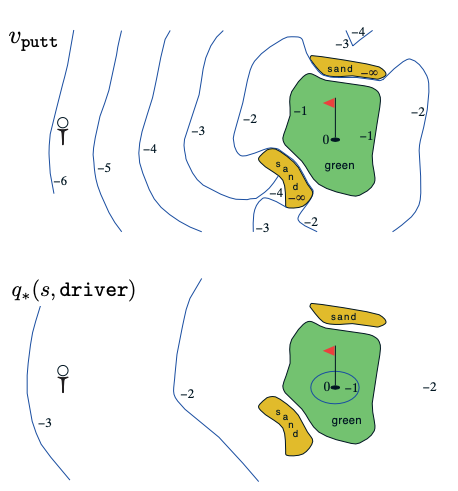
\includegraphics[width=0.5\textwidth]{/ex3.20}
	\caption{Value functions for golf.}
	\label{fig:3.20}
\end{figure}
\textbf{Q}\\
Draw or describe the optimal state-value function for the golf example.\\

\textbf{A}\\
Qualitatively, the optimal state-value function for golf (outlined by Figure \ref{fig:3.20}) would be derived from a policy that selected the driver for the first two shots (off-the green), then selected the putter for the final shot (on the green).

\subsubsection{Exercise 3.21}
\textbf{Q}\\
Draw or describe the contours of the optimal action-value function for putting, $q_*(s, \mathnormal{putter})$, for the golf example.\\

\textbf{A}\\
The optimal action-value function is given by the following:
\begin{equation}
q_*(s,a)= \sum_{s', r} p(s', r | s, a) [r + \gamma \argmax_a q_*(s,a)]\\
\end{equation}

Since we have only one action($\mathnormal{putter}$), the argmax collapses to $v_*(s')$, and $q_*(s,a) = v_*(s)$ - illustrated in Figure \ref{fig:3.20}.

\subsubsection{Exercise 3.22}
\textbf{Q}\\
\begin{figure}[h!]
	\centering
	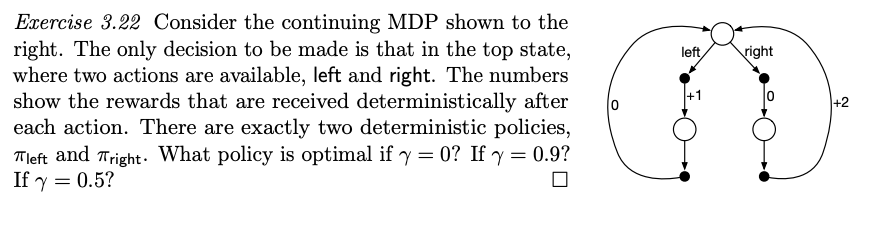
\includegraphics[width=\textwidth]{/ex3.22}
	\label{fig:3.20}
\end{figure}

\textbf{A}\\
Let's first evaluate the simplest case of $\gamma = 0$. Recall that:
\begin{equation}
v_\pi(s) = \mathbb{E}_\pi[R_{t+1} + \gamma G_{t+1} | S_t = s]
\end{equation}

For $\pi_{left}$ we get:
\begin{align}
v_{\pi_{left}} &= 1 + \mathbb{E}_{\pi_{left}} \left[0 \times \gamma G_{t+1} \right] \\
v_{\pi_{left}} &= 1 \\
\end{align}

And for $\pi_{right}$ we get:
\begin{align}
v_{\pi_{left}} &= 0 + \mathbb{E}_{\pi_{left}} \left[0 \times \gamma G_{t+1} \right] \\
v_{\pi_{left}} &= 0 \\
\end{align}

So the optimal policy for $\gamma = 0$ is $v_{\pi_{left}}$. If instead $\gamma = 0.9$, we get for $\pi_{left}$:

\begin{align}
v_{\pi_{left}} &= 1 + \mathbb{E}_{\pi_{left}} \left[0.9 \times G_{t+1} \right] \\
v_{\pi_{left}} &= 1 + \mathbb{E}_{\pi_{left}} \left[0.9 \times [r_{t+1} + \gamma G_{t+2}] \right], \\ 
\end{align}

where $G_{t+2}$ is our expected reward back at our current state. We can negate it and just look at the first loop, as max reward over first loop will create max reward in the limit. Therefore:

\begin{align}
v_{\pi_{left}} &= 1 + 0.9 \times 0 = 1,
v_{\pi_{right}} &= 0 + 0.9 \times 2 = 1.8 \\ 
\end{align}

So the optimal policy for $\gamma = 0$ is $v_{\pi_{right}}$. If, finally, $\gamma = 0.5$, we get:
\begin{align}
v_{\pi_{left}} &= 1 + 0.5 \times 0 = 1,
v_{\pi_{right}} &= 0 + 0.5 \times 2 = 1 \\ 
\end{align}

So both polices are optimal.

\subsubsection{Exercise 3.23}
\textbf{Q}\\
Give the Bellman equation for $q_*$ for the recycling robot.\\

\textbf{A}\\
$
q_*(s,a) =  \sum_{s',r} p(s',r | s, a) [r + \gamma \argmax_{a \in \mathcal{A}} q_*(s', a')]
$
where $\mathcal{A} = \{\mathnormal{search}, \mathnormal{wait}, \mathnormal{recharge}\}$

\subsubsection{Exercise 3.24}
\textbf{Q}\\
Figure 3.5 gives the optimal value of the best state of the gridworld as 24.4, to one decimal place. Use your knowledge of the optimal policy and (3.8) to express this value symbolically, and then to compute it to three decimal places.\\

\textbf{A}\\
We can observe from the grid that $\gamma = 22/24.4 = 0.9016$

Equation 3.8 was:
\begin{equation}
G_t = R_{t+1} + \gamma R_{t+2} + \gamma^2 R_{t+3} + \gamma^3 R_{t+4} + \gamma^4 R_{t+5} + \gamma^5 R_{t+6} + \ldots =  \sum_{k=0}^{\infty} \gamma^k R_{t+k+1}
\end{equation}

We can represent the optimal value function $v_*$ as:
\begin{align}
v_*(A) &= r + \gamma(v_*(A+1)) \\
 &= 10 + 0.9016(16) \\
 &= 24.426 \text{to 3 d.p.} \\
\end{align}

\subsubsection{Exercise 3.25}
\textbf{Q}\\
Give an equation for $v_*$ in terms of $q_*$.\\

\textbf{A}\\
$
v_*(s) = \max_{a \in \mathcal{A}} q_{\pi_*}(s,a)
$

i.e. returning to the diagram in exercise 3.18, $v_*$ is defined as selecting the action (in that case of a possible 3) that produces the highest state-action value function

\subsubsection{Exercise 3.26}
\textbf{Q}\\
Give an equation for $q_*$ in terms of $v_*$ and the four-argument $p$.\\

\textbf{A}\\
$
q_*(s,a) = \max \sum_{s', r} p(s', r | s, a)[r + v_*(s)]
$

\subsubsection{Exercise 3.27}
\textbf{Q}\\
Give an equation for $\pi_*$ in terms of $q_*$\\

\textbf{A}\\
The optimal policy is the one that acts greedily w.r.t the optimal state-action value function i.e. it picks the action that has the highest $q(s,a)$ in the following state.
$
\pi_*(a|s) = \max_{a \in \mathcal{A}(s)} q_*(s',a)
$

\subsubsection{Exercise 3.28}
\textbf{Q}\\
Give an equation for $\pi_*$ in terms of $v_*$ and the four-argument $p$.\\

The optimal policy is the one that acts greedily w.r.t the optimal state value function conditioned on the system dynamics
\textbf{A}\\
$
\pi_*(a|s) = \max_{a \in \mathcal{A}(s)} \sum_{s', r} p(s', r | s, a)[r  v_*(s')]
$

\subsubsection{Exercise 3.29}
\textbf{Q}\\
Rewrite the four Bellman equations for the four value functions ($v_\pi, v_*, q_\pi,and q_*$) in terms of the three argument function $p$ (3.4) and the two-argument function $r$ (3.5).\\

\textbf{A}\\
tbc







